\section{Generierung von Testdaten}
\shorthandoff{"}

%Um das Testen von Datenbank-basierten Anwendungen zu erleichtern, soll es möglich sein, automatisch Testdaten für funktionale Tests aus dem Datenbankschema generieren zu lassen. Die generierten Testdaten können direkt bzw. als Basis für die Erstellung von Testdatensätzen genutzt werden (vgl. Abb.~\ref{ansatz}). 

	\begin{figure}[tb]
		\begin{center}
			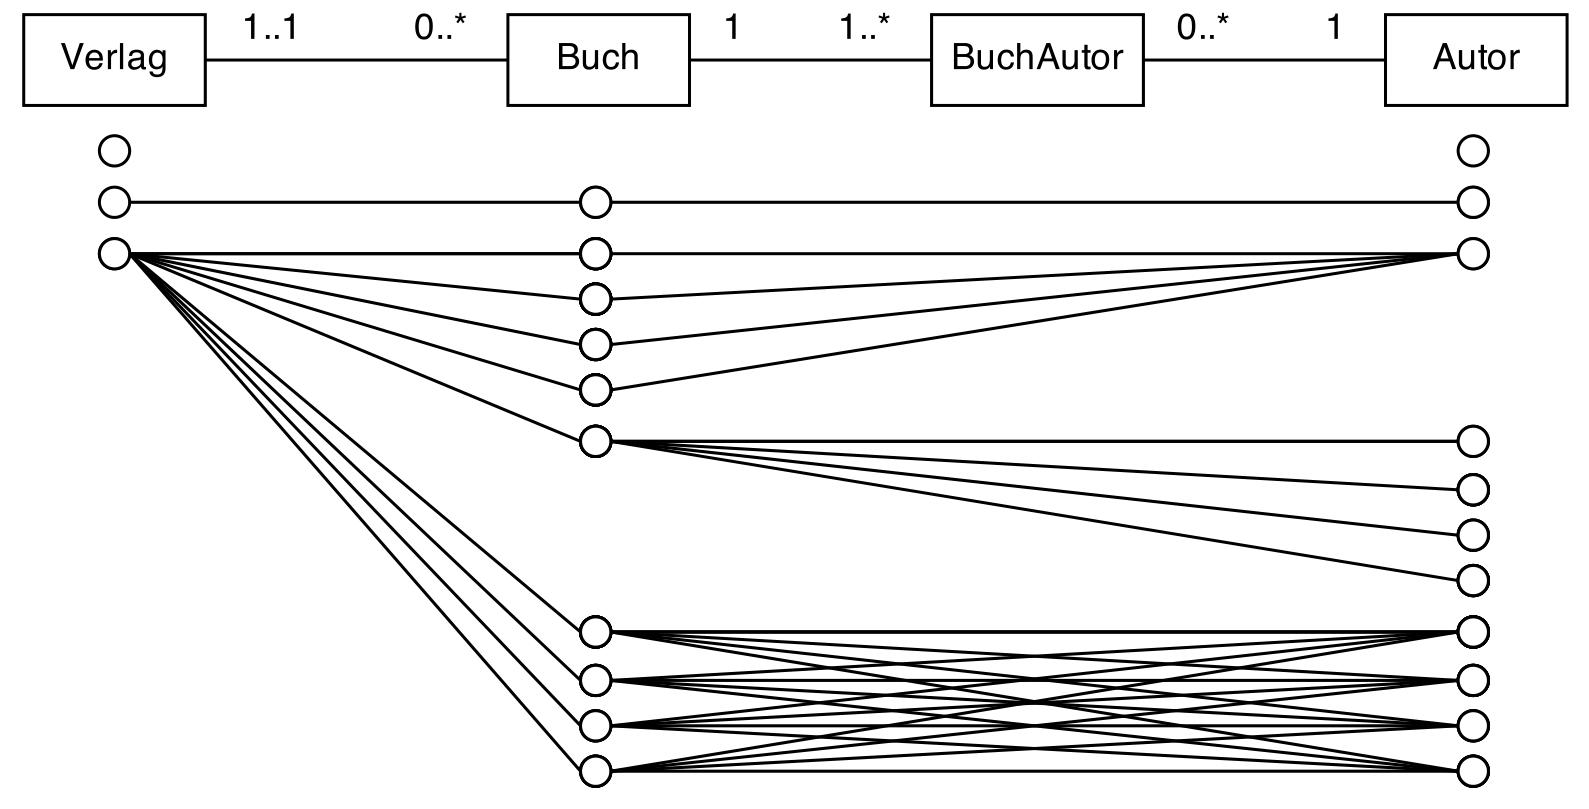
\includegraphics[width=11.5cm]{images/generiert.png}
			\caption{\label{generiert}Beispiel-Datenbankschema und daraus generierte Entitäten und Beziehungen.}
		\end{center}
	\end{figure}


Zielsetzung war die Generierung von möglichst kleinen Testdaten-Sets, die für möglichst viele fachliche Tests verwendet werden können, d.h.~eine hohe Testabdeckung bieten. 
%
%Kleine, wiederverwendbare Datasets lassen sich einfacher verstehen und erleichtern den Umgang mit Tests, da man sich  nicht immer wieder in neue Datasets hineinversetzen müssen.
%
Eine umfassende Literaturanalyse und die Evaluation existierender Werkzeuge ergab, dass bisher keine passende Lösung für diese Anforderung existiert.
%
%In der Wissenschaft beschriebene Ansätze und Algorithmen generieren meist für eine zu testende SQL-Abfrage einen passenden Testdatenbestand. Einer SQL-Abfrage liegt dabei eine formale Spezifikation zu Grunde, die allerdings für ein Anwendungsprogramm normalerweise nicht vorhanden ist. Existierende Software-Werkzeuge fokussieren sich auf die Generierung von Massendaten, die v.a. für Performanz-Tests und nicht für funktionale Tests geeignet sind. Dies zeigt sich auch daran, dass diese Werkzeuge Beziehungen zwischen Entitäten nur zufällig erzeugen und im Allgemeinen wesentlich mehr Daten generieren als für einen Menschen noch einfach verständlich sind. Weiterhin deuten Untersuchungen im Projekt darauf hin, dass die Komplexität der Testdatengenerierung im allgemeinen Fall nicht-polynomial ist.
%
Aus diesem Grund wurde ein neuer Algorithmus zur Testdatengenerierung entworfen. 
%
Anleihen konnten dabei aus \cite{Houkjaer:2006:SRD:1182635.1164254} gezogen werden.
%
Idee ist, durch Nutzung von Äquivalenz\-klas\-sen und das gezielte Generieren von Grenzfällen bei Beziehungen eine hohe Testabdeckung zu erreichen.


	




Der Algorithmus betrachtet das Datenbankschema als Graph. 
%
Tabellen stellen Knoten, Beziehungen (Fremdschlüssel) stellen Kanten dar.
%
Da assoziative Tabellen ebenfalls Beziehungen ausdrücken, werden diese als besondere Kanten behandelt. 
%
%Der Graph wird ausgehend von einem Knotens traversiert. 
%
Ausgehend von einem beliebigen Startknoten werden die Kanten und die damit verbundenen Knoten rekursiv traversiert.
%
Der Algorithmus erzeugt zu jeder Kante Entitäten der beteiligten Tabellen und mindestens entsprechend den spezifizierten Unter- und Obergrenzen Beziehungen für alle Kombinationen der unteren und oberen Grenzwerte.
%
Gleichzeitig wird versucht die Anzahl der generierten Entitäten und Beziehungen zu minimieren.
%
Aus diesem Grund werden auch nich alle --  über mehrere Kanten hinweg -- möglichen Kombinationen berücksichtigt, da dies zu einer kombinatorischen Explosion führt. 
% hier evtl die Grenzfälle erläutern...
%S
%Jede Kante und jede Tabelle werden genau genau einmal durchlaufen.
%Der  Algorithmus berücksichtigt lokal alle Kombinationen der unteren und oberen Grenzwerte von Beziehungstypen und versucht gleichzeitig die Anzahl der generierten Entitäten und Beziehungen zu minimieren. Globale Abhängigkeiten über mehrere Beziehungstypen hinweg, die zu einer kombinatorischen Explosion führen können, bleiben dabei (augenblicklich) unberücksichtigt. 


	
Der Algorithmus soll an dem  Datenbankschema  aus Abb.~\ref{generiert} (UML-Darstellung mit Multiplizitäten) veranschaulicht werden. 
%
%Ein Buch gehört genau zu einem Verlag und wird von beliebig vielen (mindestens einer) Autoren geschrieben. 
%Ein Verlag kann selbst beliebig viele und sogar keine Bücher veröffentlichen und ein Autor kann an keinem oder beliebig Büchern beteiligt sein.
%	
%	\begin{figure}[htb]
%		\begin{center}
%			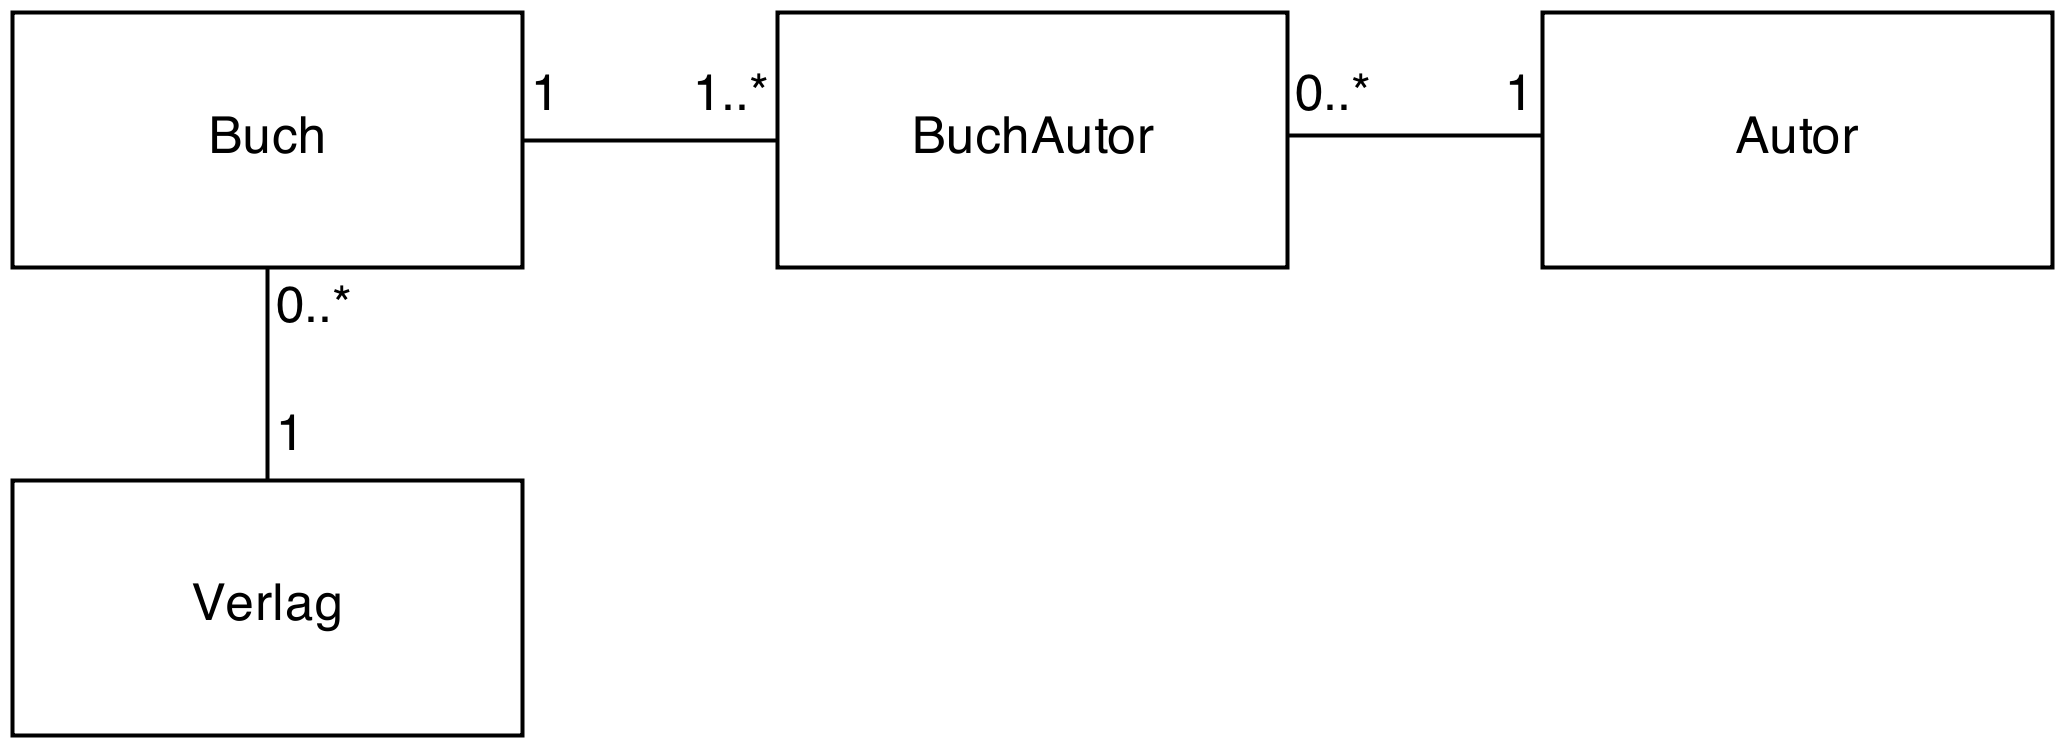
\includegraphics[width=10cm]{images/database.png}
%			\caption{\label{database}Datenbank-Schema der Bücherverwaltung}
%		\end{center}
%	\end{figure}
%	
Als Startknoten wird im Beispiel Buch verwendet. 
%
Von hier aus werden alle Kanten besucht, hier angefangen mit der Kante (1..1:0..*) zum Knoten Verlag. 
%
%Dieser repräsentiert eine 1:0..*-Beziehung. 
%
Um möglichst alle Grenzfälle bzw. Äquivalenzklassen abzudecken, wird erzeugt: (1) eine Verlags-Entität, die keine Bücher verlegt, (2) ein Verlag, der genau ein Buch verlegt und (3) ein  Verlag, der viele
Bücher veröffentlicht.\footnote{Für * wird ein konfigurierbarer Wert  verwendet, im Beispiel $4$.}
%
%Für * wird ein konfigurierbarer Wert (hier: $4$) verwendet. 
%
%Für diese Kante werden also drei Entitäten des Typs Verlag und fünf Entitäten des Typs Buch erzeugt.
%	
 Der Knoten Verlag hat keine nicht-besuchten Kanten, weshalb die Traversierung in Buch fortgesetzt wird mit der Kante zum Knoten BuchAutor (assoziative Tabelle, die eine 0..*:1..*-Assoziation zwischen Buch und Autor ausdrückt). 
%
%Die Kante hat eine assoziative Tabelle als Ziel, weshalb hier andere Schritte notwendig sind wie bei der letzten Kante.
%
%Die Tabelle BuchAutor drückt eine 0..*:1..*-Beziehung zwischen Buch und Autor aus. 
%
Der Algorithmus sieht vor, die vier möglichen min/max-Kombinationen zwischen Buch und Autor zu generieren. 
%
Jede Beziehung zwischen einem Buch und einem Autor resultiert in einer Entität in der Tabelle BuchAutor. 
%
Existierende Entitäten in Buch und Autor werden für diese generierten Beziehungen soweit möglich wiederverwendet, bei Bedarf werden neue Entitäten in Buch und Autor generiert.
%
Die Traversierung des Graph endet nun, da jede Kante besucht wurde.
%
%
%Es wird ein Autor benötigt, der kein Buch geschrieben hat, und ein Autor, der genau an einem Buch beteiligt ist (min:min). Außerdem wird ein Autor benötigt, der vier Bücher schreibt (max:min), und ein %Buch, das vier Autoren hat (min:max). Und schließlich werden vier Bücher benötigt, die jeweils die gleichen vier Autoren haben (max:max). Für die assoziative Tabelle BuchAutor werden folglich zehn Entitäten des Typs Buch und elf Entitäten des Typs Autor benötigt, wobei die bereits erzeugten Entitäten des Typs Buch hier weiterverwendet werden. 
%
%Die Traversierung endet hier, da jede Kante besucht wurde.
%
Allerdings sind einige der bis hierhin erzeugten Buch-Entitäten noch ungültig, da sie noch nicht zu einem Verlag gehören.
%
Solche Entitäten werden im letzten Schritt des Algorithmus behandelt. Alle Entitäten werden auf Gültigkeit bzgl.~ihrer Beziehungen überprüft und bei Bedarf werden weitere Beziehungen und weitere Entitäten erzeugt.
%
Abb.~\ref{generiert} stellt das im Beispiel generierte Testdaten-Set (Entitäten und ihre Beziehungen) grafisch dar. 
%
%Eine Entität wird als Kreis dargestellt, die Verbindungslinien zwischen den Entitäten stellen ihre Beziehungen dar. 
%
%Dazu gehören auch die genierten Entitäten in der assoziativen Tabelle BuchAutor.
	
%	Die fünf im vorausgegangenen Schritt erzeugten Entitäten des Typs Buch sind allerdings noch ungültig, da sie noch nicht zu einem Verlag
%	gehören. Solche Entitäten werden im letzten Schritt behandelt. Alle Entitäten werden auf Gültigkeit bzgl. ihrer Beziehungen überprüft,
%	und bei Bedarf werden weitere Beziehungen und falls notwendig weitere Entitäten erzeugt. Abb.~\ref{generiert} stellt die generierten
%	Entitäten und ihre Beziehungen grafisch dar. Eine Entität wird als Kreis dargestellt, die Verbindungslinien zwischen den Entitäten
%	stellen ihre Beziehungen dar. Dazu gehören auch die genierten Entitäten in der assoziativen Tabelle BuchAutor.
		
Details zum Algorithmus (Pseudocode) und zur Java-Implementierung sind in \cite{MT:Moll:2013} zu finden.
%
Evaluationen haben gezeigt, dass die generierten Testdaten unabhängig von der Reihenfolge der Traversierung und  bzgl.~des Datenbankschemas immer gültig sind.
%
Zur Erzeugung der Werte von Entitäten wurden verschiedene Wertegeneratoren implementiert.	

%	Der Algorithmus wurde in Java als Teil von STU implementiert. Details zum Algorithmus und sein Pseudo-Code, zur Implementierung und zur
%	Generierung von Daten für die einzelnen Entitäten sind in \cite{MT:Moll:2013} zu finden. Verschiedene Evaluationen haben gezeigt, dass
%	sich die erzeugten Testdaten in Unit-Tests nutzen lassen und auch in die Datenbank einspielen lassen. Das Ergebnis der Generierung ist
%	bei der aktuellen Implementierung unabhängig von der Reihenfolge der Traversierung.
	
	

